%!TEX TS-program = xelatex
%
% Created by Snow on 2017-11-14.
% Copyright (c) 2017 .
\documentclass[11px]{article}

%\usepackage{polyglossia}
\usepackage{hyperref}
\usepackage{xspace}
\usepackage{amsmath}
\usepackage{graphicx}
\usepackage[a4paper, top=1in, bottom=1in, left=1in, right=1in]{geometry}
\usepackage{comment}


\newcommand{\projTitle}{BitMesh\xspace}

\title{COMP6111C Project Proposal}
\author{Justinas LINGYS, 20082250 \\ Junxue ZHANG, 20371613}
\date{}

\begin{document}

\maketitle

\abstract{With the increasing popularity of cloud computing, users begin to deploy more critical services and applications on the cloud. To ensure high availability and reliability, monitoring and diagnostic systems have become an important components for both cloud providers and users. However, currently, either deployed by the providers or users, those systems are not optimal. For cloud providers, they incur extra resource consumption and lack the ability to access user deployed application logs or status. For users, lack of global information restricts the effectiveness of the system. To solve this, we propose \projTitle. \projTitle leverages the block chain data structure and uses proof-of-statistics to increase the resource utilization. In the system, the cloud provider acts as the regulator of the system and the miniers are volunteers from the users. Via our evaluation with scalability and performance, we understand how \projTitle can scale when the number of nodes increases. By comparing the value of information collected, \projTitle can largely outperforms the traditional monitoring and diagnostic systems due to its ability to access information from both physical and virtual machines.}

\section{Introduction}
The public cloud, such as Amazon EC2\cite{url/ec2}, Microsoft Azure\cite{url/azure}, etc., has been an ideal place for users to host their applications in recent years. The cloud computing dramatically benefit those users by providing low cost and pay-for-use computation resources, such as virtual machines (VMs). Users rent VMs from cloud service provider and deploy their applications inside VMs, such as web servers for HTTP request, FTP servers for file sharing and so on. With the increasing popularity of cloud computing, users begin to deploy some critical applications or services, such as financial analytical service or human resource management systems, on the cloud. How to guarantee that those services or applications will not fail accidently poses great challenges for both cloud providers and users. Traditionally, by deploying a monitoring and diagnostic system, it can mitigate the risk of those grey failure, but we will show in the following parts that it is not easy and optimal for either the cloud provider or the users to deploy such an monitoring and diagnostic systems.

\textbf{For cloud providers.} Cloud providers usually deploy some monitoring and diagnostic applications in their cloud data centers. The monitoring and diagnostic system collect data from either network or endhost and use those data to detect failure, analyze root cause and trigger troubleshooting reports. Trumpet\cite{sigcomm/trumpet} is a typical tool deployed on endhost to collect flow information, such as source/destination address to predict or report potential congested point. However, to make the Trumpet fully function, CPU, memory and bandwidth at endhost will be consumed, which is not desirable in cloud data centers where all resources are expected to be allocated for users. NetPoirot\cite{sigcomm/netpoirot} is another endhost based solution and captures TCP statistics to identifies the root cause of failure using the information at a single endhost. Both of those endhost based solution suffer from \textbf{extra resource consumption}, which indirectly \textbf{reduces the profit for cloud providers}.

Another category of monitoring and diagnostic system is to collect data from network instead of endhosts. These methods usually require the support from the switches, such as NetFlow\cite{url/netflow} and sFlow\cite{url/sflow}. A more recent and advanced work is Marple\cite{sigcomm/marple}, which designs and implements a hardware-specific query language to efficiently query the switch status to infer the whole network system. To adopt those in-network monitoring and diagnostic system, cloud provider should use some \textbf{advanced network switches}, which also increases the operational cost for cloud data centers.

Moreover, for cloud providers, all data collected is from physical machines or network. However, those data cannot reflect the status inside the virtual machines, which are not efficient in detecting user's problem. As a result, it may be very \textbf{difficult for cloud providers to provide accurate and effective monitoring and diagnostic service for users}.

\textbf{For users.}
Users can deploy his own monitoring and diagnostic system inside all his virtual machines to provide high availability. One example is users can deploy Ganglia\cite{url/ganglia} inside all their virtual machines. Ganglia will collect data from all virtual machines owned by the user and generate status report for users. Users can know the real-time status and predict the potential failure based on those report. However, in public cloud data centers, all computation resources are shared among the users. Virtual machines owned by different users may be placed on the same physical machines\cite{infocom/lets_stay_together}. It would further benifit the monitoring and diagnostic if you can get the information from other virtual machines that has been placed together with your virtual machines. Here is an example: if 10 VMs are placed on 1 physical machine and you only own one of them, when you see your application generates more error logs, you cannot tell whether the VMs has potential problems or it is just some accidental case. However, if you can access the application-level data of the other 9 VMs, when you observe that most of them experience a high error rate, we can tell with high confidence that the physical machine may have some problems and thus we should not use the VMs on this physical machines currently or report to the cloud provider. For users, \textbf{lack of global information in the whole cloud data centers} limit the effectiveness and accuracy of their monitoring and diagnostic systems.

In conclusion, current monitoring and diagnostic systems in cloud data centers, either deployed by cloud providers or service users, suffer from the following drawbacks:

For cloud providers:
\begin{itemize}
	\item Extra resource waste. Monitoring and diagnostic systems consume plenty of resources, which indirectly reduces the profit of cloud provider.
	\item Lack of application-level information. Due to privacy concern, cloud providers cannot directly access application-level information inside VMs, which acts an quite important role in monitoring and diagnostic.
\end{itemize}

For users:
\begin{itemize}
	\item Lack of global information. Users can only access the data from the machines that he owns. Lack of global information leads to suboptimal monitoring and diagnostic results.
\end{itemize}

In this project, we are taking one step back and wondering whether it is possible to combine the advantage of both two solutions and mitigate the above problems. The answer is \projTitle.

\projTitle leverages the block-chain data structure and motivates users to participate in the system. \projTitle uses proof-of-statistics(\S~\ref{sssec:proof_of_statistics}) instead of proof-of-work to benefit the resource utilization. The cloud provider can also act as a central entity to regulate the whole system, which is not mandatory in our design.

We show later in this project report, \projTitle can meet the following design goals:

\begin{itemize}
  \item No resource consumption for cloud provider. All computation resource needed in monitoring and diagnostic are provided by users but not cloud provider.
  \item Access to application-level information. We are not restricted to only use the information from hypervisor but from user-deployed applications.
  \item Access to global information. The monitoring and diagnostic system use data from all users to generate report for each user.
  \item Safety and security. We should satisfy some security and safety requirements. Such as user can access his own report; the system could prevent attack from malicious users.
\end{itemize}

\begin{comment}
\section{Methodology}
\subsection{Overview}
Figure~\ref{} shows the overall design of \projTitle. There are three roles in the system, the central entity, the miners and the users. The central entity can be the cloud provider, which is not mandatary. The central entity is only responsible for regulating the system, such as selecting miners. The miniers are volunteers from users, which provide the computation resource to generate monitoring or diagnostic reports for users. To motivate users to become miners, miners can access the global information of the data center. We believe lots of research institutions and labs will be interested in those data and participate in the system, which would in turn benefit the whole community. The normal users are required to send his application-level logs or status to miniers for generating the monitoring or diagnostic models. Users are rewarded by a more frequent monitoring or diagnostic reports if he sends his logs more frequently to the whole system.

\subsection{Proof-of-Statistics}
\label{sec:proof-of-statistics}
Proof-of-work has been identified as a major bottleneck of scalability of \textit{Bitcoin}  and has been tackled by replacing it with some useful work \cite{filecoin-storage} or with a new system architecture \cite{RSCoin-bank}.  Replacement of proof-of-work with some
efficient actions in blockchain-based systems can bring a great number of benefits since the usually wasted resources aggregate to an enormous amount of  computational power \cite{bitcoin-comp-elec-power}. Cloud data centers are not an exception for such an
improvement. Data center environments are usually highly optimized and any system resource wastage is considered as critical and intolerable \cite{google-ai-power, facebook-cold-storage-rack}. Due to such stringent data center requirements, in-data center services
shall not incur any overhead on the miners for maintaining a globally shared blockchain and shall not result in misuse of CPU or any other resource. Considering this, we propose a paradigm called 'Proof-of-Statistics', which employs the miners as ordinary computation nodes
for performing statistical operations on received data. The CPUs and other resources are dedicated to actions that are extensively conducted in modern data centers \cite{microsoft-autopilot} and which provide the miners with a reward.
\end{comment}

\section{System Architecture and Proof-of-Statistics}
Proof-of-work has been identified as a major bottleneck of scalability of \textit{Bitcoin}  and has been tackled by replacing it with some useful work \cite{filecoin-storage} or with a new system architecture \cite{RSCoin-bank}.  Replacment of proof-of-work with some
efficient actions in blockchain-based systems can bring a great number of benefits since the usually wasted resources aggreate to an enormous amount of  computational power \cite{bitcoin-comp-elec-power}. Cloud data centers are not an exception for such an
improvement. Data center environements are usually highly optimized and any system resource wastage is considered as critical and intolerable \cite{google-ai-power, facebook-cold-storage-rack}. Due to such stringent data center requirements, in-data center services
shall not incur any overhead on the miners for maintaining a globally shared blockchain and shall not result in misuse of CPU or any other resource. Considering this, we propose \textit{\projTitle}, a distributed system for employing the miners as ordinary computaion nodes for performing statistical operations on performance metrics of data center clients. The CPUs and other resources are dedicated to actions that are extensively conducted in modern data centers \cite{microsoft-autopilot} and which provide the miners with a reward - realistic data center characteristics. \textit{\projTitle} assumes that the miners are willing to dedicate their resources for collecting performance data from data center clients for personal use (research purposes) or for providing a service for the clients to improve their own infrastructure wthough a global view of the entire facility.

The rest of the section will describe the architecture of the system in \S\ \ref{ssec:system_design_and_flow} and will explain
the processing of data at miners in \S\ \ref{ssec:work_of_miners}.

\begin{figure}[h!]
  \begin{center}
    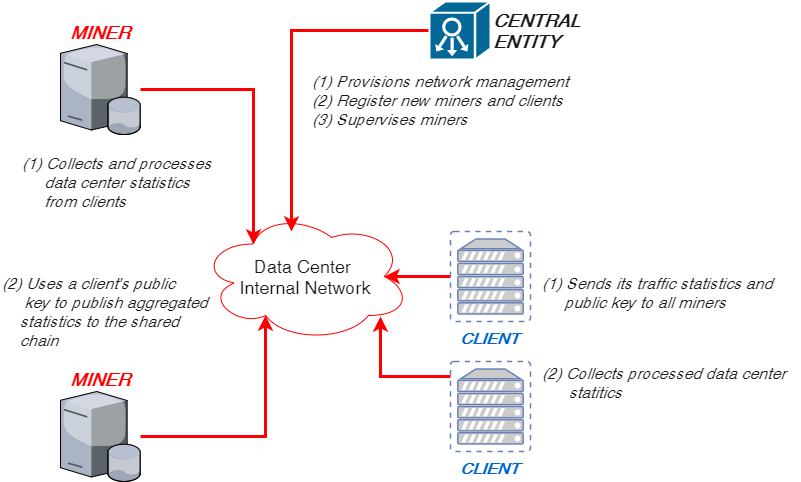
\includegraphics[width=0.8\linewidth]{figures/project_design.png}
    \caption{High-level Design of \textit{\projTitle}}
    \label{fig:project_design}
  \end{center}
\end{figure}

\subsection{Data Flow and System Participants}
 \textit{Bitcoin} has applied a design of a globally shared ledger for recording all the transactions occurred in the system \cite{bitcoin_paper}. Such a design introduces differentiation between system nodes: \textit{miners} and \textit{currency users}. As though, despite its architectural issues and performance problems, \textit{Bitcoin} remains a global peer-to-peer network which is used by many users every day. Thus, it appears reasonable to adhere to the original proposal of \textit{Bitcoin} and segregate \textit{minders} from \textit{clients}. The proposed system, \textit{\projTitle}, exploits the fundamental principles of \textit{Bitcoin} with an extra entity: central controller, which, in data centers, may be the administrator of the data center (Figure \ref{fig:project_design}). The role of the central entity is minimal and is not crucial to implement the system. Though having a reliable controller unit simplifies the system and provides security benefits. The section will briefly explain the roles of each of the entities of the system and will describe a data processing path in the rest of the section.

\paragraph{Central Entity (Controller):} The role of the central entity is more administrative than system-crucial. Many cloud data centers employ central control units for controlling system updates \cite{microsoft-autopilot}, data flows \cite{google_jupiter}, or system errors \cite{microsoft_netpoirot}. \textit{\projTitle} relies on a centralized controller for admitting new miners/clients to the system. Such an approach is chosen as currently most data centers do not support multicast packets and it is relatively expensive to flood a data center network in order to get approved as a new miner or a client. Hence, having a well-know service reduces system complexity and ensures that no data center bandwidth is wasted for just transmitting registration packets. The central entity accepts a new client and provides it with enough information about the current miners (miner IP addresses and their public encryption keys) so that it can become a part of the global ecosystem (Figure \ref{fig:central_entity_client_reg}). After retrieving the needed information, the client directly interacts with miners to have its work processed and stored. Due to this, the involvement of the central entity is minimal and does not require any computationally-intensive operations for handling client requests. Scalability is considered in the design and should not be an issue as similar systems exist in real deployments \cite{hadoop_example}. The work assumes that a commodity server should suffice for running the service in most cloud data centers.

\subsection{Data Flow and System Participants} \label{ssec:system_design_and_flow}
 \textit{Bitcoin} has applied a design of a globally shared ledger for recording all the transactions occured in the system \cite{bitcoin_paper}. Such a design introduces differentiation between system nodes: \textit{miners} and \textit{currency users}. As though, despite its architectural issues and perforamnce problems, \textit{Bitcoin} remains a global peer-to-peer network which is used by many users every day. Thus, it appears reasonable to adhere to the original proposal of \textit{Bitcoin} and segregate \textit{miners} from \textit{clients}. The proposed system, \textit{\projTitle}, exploits the fundamental principles of \textit{Bitcoin} with an extra entity: \textit{central controller}, which, in data centers, may be the administrator of the data center (Figure \ref{fig:project_design}). The role of the central entity is minimal and is not crucial to implement the system. Though having a reliable controller unit simplifies the system and provides security benefits. The subsection will briefly explain the roles of each of the entities of the system and will describe communication flow between the system entities.


\begin{figure}[h]
  \begin{center}
    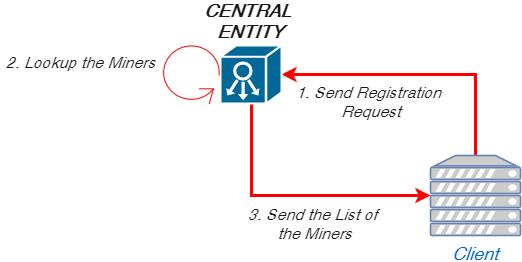
\includegraphics[width=0.6\linewidth]{figures/central_entity_client_reg.png}
    \caption{Central Entity-Client Interaction}
    \label{fig:central_entity_client_reg}
  \end{center}
\end{figure}

\paragraph{Central Entity (Controller):} The role of the central entity is more administrative than system-crucial. Many cloud data centers employ central control units for controlling system updates \cite{microsoft-autopilot}, data flows \cite{google_jupiter}, or system errors \cite{microsoft_netpoirot}. \textit{\projTitle} relies on a centralized controller for admitting new miners/clients to the system. Such an approach is chosen as currently most data centers do not support multicast packets and it is relatively expensive to flood a data center network in order to get approved as a new miner or a client. Hence, having a well-know service reduces system complexity and ensures that no data center bandwidth is wasted for just transmitting registration packets. The central entity accepts a new client and provides it with enough information about the current miners (miner IP addresses and their public encryption keys) so that it can become a part of the global ecosystem (Figure \ref{fig:central_entity_client_reg}). After retrieving the needed information, the client directly interacts with miners to have its work processed and stored. Due to this, the involvement of the central entity is minimal and does not require any computationally-intensive opeartions for handling client requests. Scalability is considred in the design and should not be an issue as similar systems exist in real deployments \cite{hadoop_example}. The work assumes that a commodity server should suffice for running the service in most cloud data centers.
\par


\noindent \newline On the other hand, the controller is also reponsible for approving new miners and supervising their integration into the current pool of miners. A new miner receives a list of the current miners $L$ and an approval certificate $Cr$ from the central entity.
The approval certificate $Cr$ is signed by the central entity to ensure other miners that the newcomer has been approved to be a miner \cite{public-auth-certificate}.


\paragraph{Clients:} Generating local system statistics (observing data flow latencies, thoughput, CPU utilization, and etc.) is prevalent in cloud data centers. However, clients of a cloud data center can only be in charge of their own systems and are rather oblivious to the overall data center network. Despite storage of local system logs, measurements, the clients cannot go beyond their virtual networks (VNs) and are left with the locality drawback. Clients of \textit{\projTitle} can share their local statistics with the miners and get access to a more concise view of the entire network. A client is required to register for membership with the central entity (Figure \ref{fig:central_entity_client_reg}), and then directly communicate with the miners to send its local information about its system to the miners. The work assumes the clients are always honest and share their uncompromised information. However, if a client is dishonest and sends modified information to the miners, it may be identified as inconsistent and the client may lose its membership due to compromised statistics (\S\ \ref{ssec:work_of_miners}).

\noindent \newline Furthermore, clients use a popular teqchine the power of two choices \cite{power_of_two_choices} for selecting  miners. A Client query two random miners and chooses the one out of two with lower load (lower CPU utilization, memory utilization, shorter request queue). There is no incentice for the miners to lie about its load since eventually all miners receive the same information about active clients.s
\par

\paragraph{Miners:} Collecting various system metrics from clients and producing a concise summary for the clients in a form of a aggreagted log.The miners are the core of the system and take similar reponsibilities to the ones in \textit{Bitcoin} (Figure \ref{fig:miner_work_flow}). The major responsibility of the miners is to process system metrics in a required manner.The miners define a set $O$ of operations that they are capable of applying on particular data from a set $M$. Clients must be aware of the sets and only requests that comply with the both sets are processed by the miners. A request from a client is processed as it it described in \S\ \ref{ssec:work_of_miners} and the result of the request is shared among all the miners for voting and approval. Such a step is needed to ensure that all miners have the same information and that 'lazy' miners would be identified and removed from the set of the current miners. The loss of membership in the current set of miners is not the major contribution of the work, so it is not described in detail. A miner can lose its membership if other miners observe that the miner of interest is not contributing enough of its processing power. Each miner has to be aware of the other miners and keep track of a set $R_{miners} = \{r_1, ..., r_n\}$ which stores approximate rates, of  miners' result publishing. If a rate, $r_i$, goes below a value $m_{miner}$,  for example, lower quartile of all rates in the set $R_{miners}$ or some fixed percent below the mediate value of all rates, miners vote for removing a particular miner $i$ from the current miners. If the vast majority of the miners agree on the removal of a miner $i$,  the central entity must be informed about such a result so that the central entity would store the latest set of the current miners.
\par


\begin{figure}[h]
  \begin{center}
    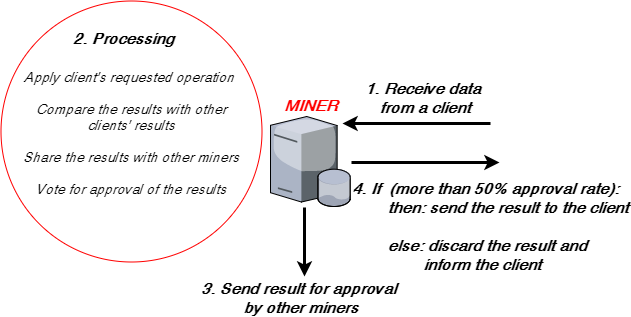
\includegraphics[width=0.8\linewidth]{figures/miner_work_diagram.png}
    \caption{Flow of a Miner's Work}
    \label{fig:miner_work_flow}
  \end{center}
\end{figure}


\subsection{Work of Miners}\label{ssec:work_of_miners}
Miners dedicate their computational power to process client requests and aggregate statistical information from all the requests. The processed information is stored in a blockchain-based ledger and each new block is only appended to it if more than $50\%$ of current miners approve it. Also, the blockchain naturally provides a timestamp sequence which is important to computation and inference since data center workloads experience diurnal patterns \cite{diurnal_pattern_data_center_1, diurnal_pattern_data_center_2}. The rest of this section will focus on the statistical computation of a request (\S\ \ref{sssec:proof_of_statistics}) and how a client can be identified as a malicious one in some cases (\S\ \ref{sssec:malicious_client}).

\subsubsection{Proof-of-Statistics}\label{sssec:proof_of_statistics}
As mentioned before, the miners of \textit{\projTitle} process the requests from clients in statistical manner and computes statistical metrics as a result. The process of handling a request is called \textit{Proof-of-Statistics} since a miner does useful work to create a new block of the blockchain. Different statistics can be  computed on different performance metrics, $O$, on the provided data. Due to space limitation, this section only focuses on flow completion times (FCTs) and network throughput since these two metrics are among the most important ones for networking.

\noindent \newline A client shares with a miners its FCTs, traffic matrix, and throughput together with hardware specifications such as NIC Capacity, number of cores, and others. The miner applies an operation $o \in O$ on the data, computes statistics of the data, $S_{sample} = \{s_1, ..., s_k\}$, and updates the results of the corresponsing global values $S_{global} = \{g_1, ..., g_k\}$.
The computed statisitcs are first checked for compliance with the global values (\S\ \ref{sssec:malicious_client}) to filter out malicious clients before updating the global values, $S_{global}$. However, as it has been mentioned before, this step is optional since \textit{\projTitle} assumes honest clients.

\subsubsection{Malicious Clients}
\label{sssec:malicious_client}
\textit{\projTitle} assumes honest clients, but includes an optional step in the acceptance of a request. Since each of the miners stores the global infomration, it is easy for each of the miner to retrieve the global statistics of all clients, $S_{global}$. After computing the statistics of a recieved request, $S_{sample}$, the responsible miner can compare them with the corresponing global ones. Hypothesis testing or known distribution fitting \cite{walpole_statistics} are considered as powerful enough tools to detect extremely malicious clients. It is well-known that data center workloads follow long-tailed distributions \cite{diurnal_pattern_data_center_2, dctcp_ref, pFabric_ref}, so such a fact can make it easier to detect dishonest clients.

\subsection{Approval of a New Result}
As it is shown in (Figure \ref{fig:miner_work_flow}), a miner has to share its computation with the rest of the miners.  This step is required so that other miners could update their shared information and also check if the new request is not from a 'lazy' miner (\S\ \ref{ssec:system_design_and_flow}). A miner, $i$, is capable of  reusing an old processed request from a client in order to ensure a high publishing rate, $r_i$. \textit{\projTitle} uses a simplistic method of checking for miner's reliability since the work assumes that miners should not have high incentice to compromise the global information since the information is supposed to be used by the miners for their personal work (e.g., researcher may use the collected data for their publications).

\noindent \newline A set of other miners, $A= \{a_i, ..., a_t\}, \; \; where \; \; |A| > 50\% \; \; of \; \; miners$ , query the client whose request has been processed by the miner $i$. If the client has no pending requests or its pending requests have different sequence numbers, $Seq$, then the miners reject the processed request. If the request is approved, each of the miners update the publishing rate, $r_i$, and the global information (approves the request).

\noindent \newline After the voting step, the miner $i$ sends an encrypted block $B_{ecr}$ by using a public key,$pr_j$ , to the client $j$, who has sent the request for processing. The block, $B_{ecr}$, contains processed request together with global data $S_{global}$  and other related information to $S_{global}$.

\section{Evaluation}
In this evaluation section, we are going to answer the following questions:

\begin{itemize}
  \item How does \projTitle scale when the number of users/miners are increasing ? \\
      Evaluation was performed to show the communication overhead of \projTitle when the number of nodes(both miners and users) increases. (\S~\ref{ssec:eval_scalability})
  \item How does \projTitle perform compared to the systems deployed either by users and cloud providers in accuracy and efficiency ? \\
      \projTitle can largely outperform exiting solutions by gaining the access to both user-level and global information. (\S~\ref{ssec:eval_performance})
\end{itemize}

\subsection{Methodology}
We use Python to execute our simulations. For scalability evaluation, we are evaluating the message complexity when the number of users/miners increase. We capture the message sent during the whole monitoring and diagnostic process. For performance comparison. We compare \projTitle with systems deployed by cloud providers and users respectively. We use the information value $V$ to denote the value of information collected by the whole system. In this evaluation, we assume we have 1000 physical machines, each contains around 4 virtual machines. One user owns around 20 virtual machines. The information generated in the VMs are more valuable compared to the information generated from the physical machines (hypervisors).

\subsection{Scalability}
\label{ssec:eval_scalability}
A diagnostic system has to scale to a large number of nodes. Due to this, \projTitle has been evaluated in terms of the number of generated messages in the system (system workload) at different numbers of miners and clients (Figure \ref{fig:complexity_measure}). The graph shows the number of messages generated in the system when each client generates a request. The rate of the request is not considered in the graph since it is not easy to approcimate such a values, however, it has been reported that traditional very large data centers collect performance metrics from the servers once a few seconds \cite{microsoft-autopilot} in order to avoid overloading the network. The overall number of messages generated per request provides a rough idea about how much work the miners would to handle without mining, only for communication. We leave the more thorough evaluation for future work as it may require extra system resources.

\begin{figure}[h]
\centering
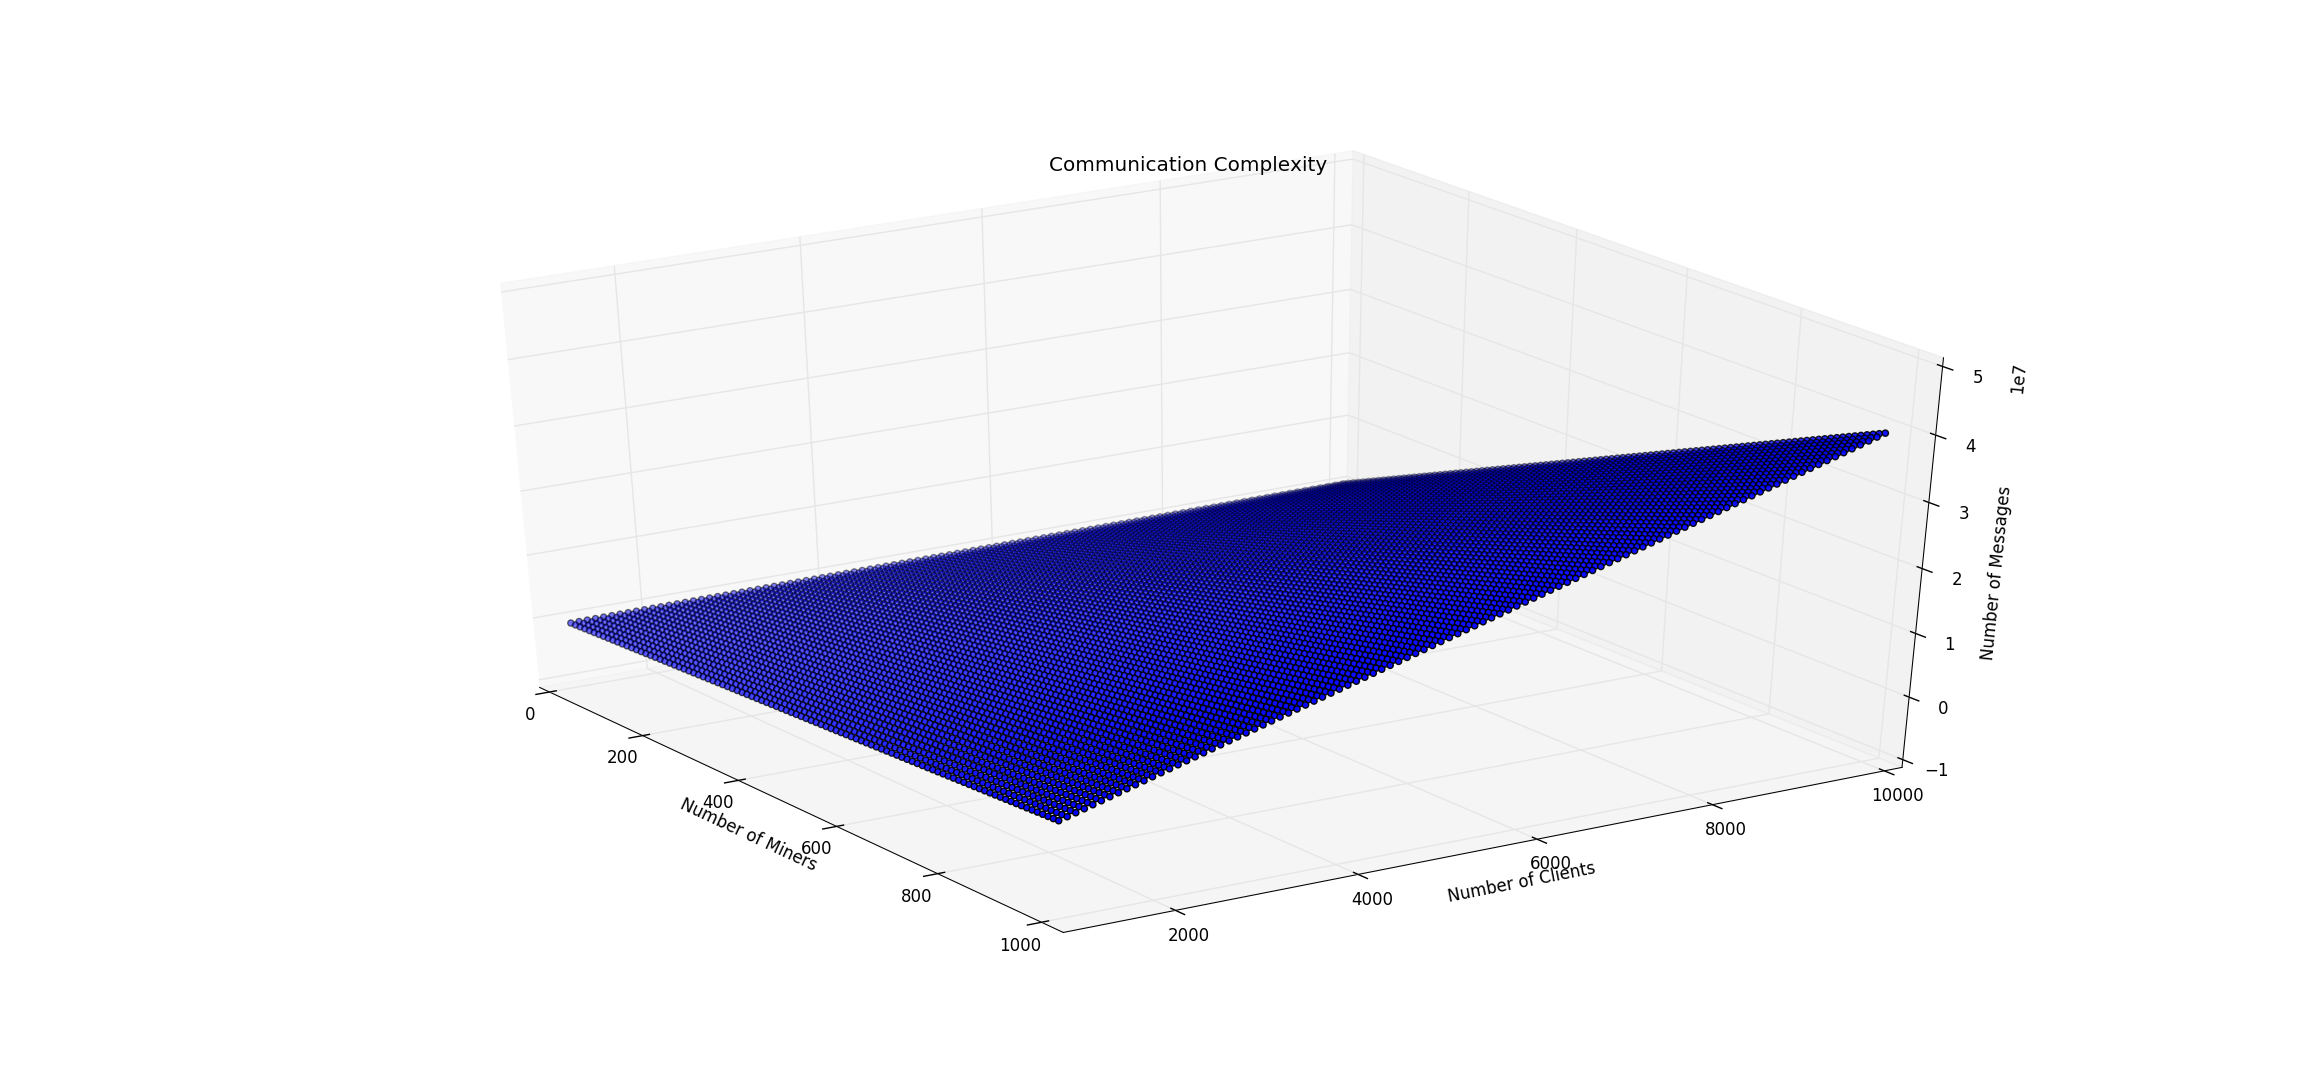
\includegraphics[width=0.8\linewidth]{figures/complexity_of_communication.png}
\caption{Communication Complexity of \projTitle in terms of generated messages.}
\label{fig:complexity_measure}
\center
\end{figure}

\subsection{Performance comparison}
Figure~\ref{fig:performance} shows the results of performance comparison among \projTitle, system deployed by the users and the system deployed by the cloud providers. We observe that the system deployed by the users get the lowest valuable information since users can only access their own virtual machines. Lack of global information has lead to suboptimal performance for users. Furthermore, system provided by the cloud provider is also $~20\times$ worse than \projTitle due to the lack of user-level information. \projTitle achieves the best performance by combining both the information from physical machines and virtual machines, and large outperforms the other two systems.

\label{ssec:eval_performance}
\begin{figure}[h]
\label{fig:performance}
\center
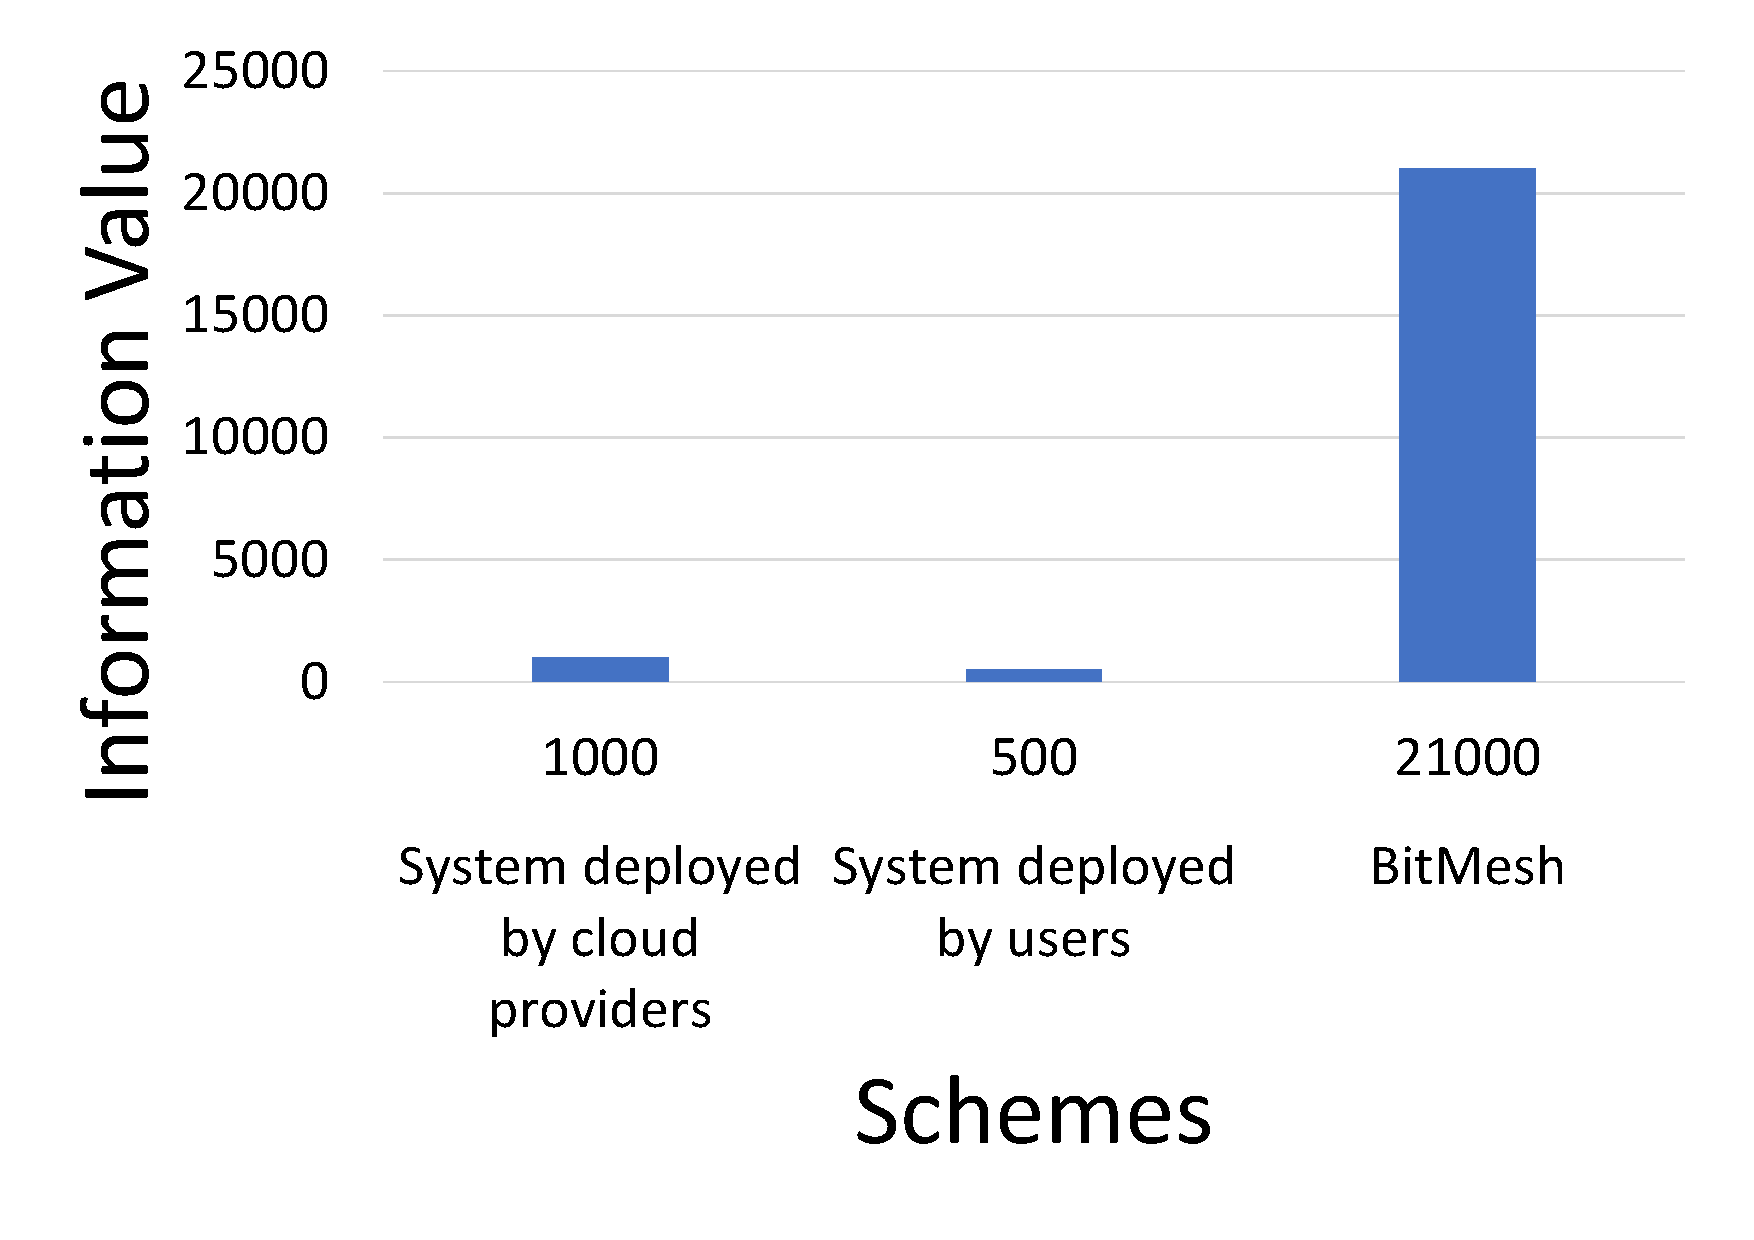
\includegraphics[width=0.6\linewidth]{figures/peformance.pdf}
\caption{Performance of \projTitle compared with systems deployed either by cloud providers or users. The \projTitle gains the most information value because it can access both the user-level application logs and global information.}
\label{fig:miner_work_flow}
\end{figure}

\section{Conclusion}
We propose \projTitle in this report, which mitigates the drawbacks of systems both deployed by the cloud providers or users. We also perform Python based simulations to show that \projTitle have good scalability. Moreover, by gaining the access to both application-level logs and global information, \projTitle can largely outperform the existing monitoring and diagnostic systems. \projTitle has the potential ability to play big as the novel monitoring and diagnostic systems in cloud data centers.

\newpage
\bibliographystyle{IEEEtran}
\bibliography{proposal}

\end{document}

